A motor position control system with controller, disturbance, and sensor is shown in the figure below. 
\begin{center}
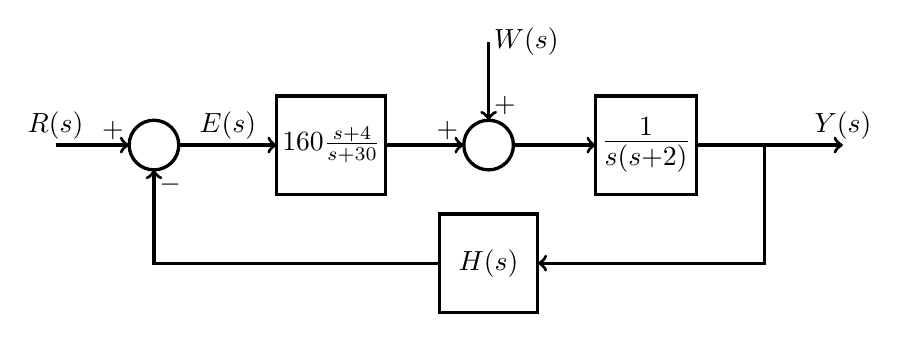
\begin{tikzpicture}[scale=1,inner sep=0pt,outer sep=0pt,very thick,
sysblock/.style={draw,rectangle,inner sep=2pt,minimum width=1.25cm,minimum height=1.25cm,very thick}]
\draw (1.75,0) node[draw,circle] (sum1) {$\rule{0pt}{18pt}$};
\draw (4,0) node[sysblock] (Kp) {$160 \frac{s+4}{s+30}$};
\draw (6,0) node[draw,circle] (sum2) {$\rule{0pt}{18pt}$};
\draw (8,0) node[sysblock] (G) {\Large $\frac{1}{s(s+2)}$};
\draw (6,-1.5) node[sysblock] (H) {$H(s)$}; 
%\draw[->] (.5,0) node[above=2pt] {$R(s)$} -- (sum1.180) node[above left=2pt] {$+$};
\draw[->] (.5,0) node[above=2pt] {$R(s)$} -- (sum1.180) node[above left=2pt] {$+$};% (1,0) node[above right=2pt] {$E(s)$};
\draw[<-] (sum2.90) node[above right=2pt] {$+$} -- ++(0,1) node[right=2pt] {$W(s)$};
\draw[->] (sum1.0) -- node[pos=.5,above=2pt] {$E(s)$} (Kp);
\draw[->] (Kp) -- (sum2.180) node[above left=2pt] {$+$};
\draw[->] (sum2) -- (G);
\draw[->] (G) -- ++(2.5,0) node[above=2pt] {$Y(s)$};
\draw[->] (G) ++(1.5,0) |- (H);  
\draw[->] (H) -| (sum1.-90) node[below right=2pt] {$-$}; 
\end{tikzpicture}
\end{center}
Note that the error signal $E(s) = R(s)-H(s)Y(s)$ is defined specifically for this application and is not a universal definition when the feedback path is non-unity.
\begin{enumerate}
\item Assume that the sensor is perfect; that is, $H(s)=1$.  Determine if the system can reject a unit step disturbance $w(t)$ with zero steady-state error.  If the answer is no, determine the steady-state error to this disturbance.
\item Assume that the sensor dynamics are given by $H(s) = \frac{20}{s+20}$.  Determine if the closed-loop system can reject a unit step disturbance $w(t)$ with zero steady-state error.  If the answer is no, determine the steady-state error to this disturbance.
\item Using \textsc{Matlab} and the \texttt{step} command, simulate the system for cases $(a)$ and $(b)$ (with $r(t)=0$) to verify your answers. For full credit, include the Matlab plots. 
\end{enumerate}
